\documentclass[12pt, a4paper]{article}

%******************* Importado Pacotes *********************************************

\usepackage[brazil]{babel}
\usepackage[pdftex]{graphicx}
\usepackage[ansinew]{inputenc} % permite acentua��o correta
\usepackage{times}    
\usepackage{setspace} 
\usepackage{xspace}   
\usepackage{float}
\usepackage{color}
\usepackage{colortbl}
\usepackage{verbatim}
\usepackage{textfit}
\usepackage{multirow}
\usepackage{alltt}
\usepackage[T1]{fontenc}
\usepackage[verbose,left=25mm,right=25mm,top=30mm,bottom=30mm]{geometry} % margens
\usepackage{ae}
\usepackage{fancyhdr}
\usepackage{fancybox}
\usepackage{multicol}
\usepackage{listings}

\usepackage{placeins} 
\usepackage{url}
\usepackage[%numbers,
            authoryear,
            sort&compress,]{natbib}
\usepackage[compact]{titlesec}  
%\usepackage[pdftex]{hyperref}  % gera os hiperlinks no pdf

\usepackage[pdftex,plainpages=false]{hyperref}

\hypersetup{colorlinks=true,debug=false,
  linkcolor=black,%%%cor do tableofcontents,\ref,\footnote,etc
  citecolor=black, %%% cor do \cite
  urlcolor=black, %%% cor do \url e \href
  pdftitle={Gerador de aplica��o Captor},
  pdfauthor={Edison Kicho Shimabukuro Junior},
  pdfsubject={Gerador de aplica��o Captor}}

\pdfcompresslevel=9
\DeclareGraphicsExtensions{.png,.jpg,.pdf,.mps} 


%*****************************  Definicoes de estilo   ************************

%\let\chapter=\section
%\let\section=\subsection
%\let\subsection=\subsubsection

%\let\cite=\citep
%\let\ingles=\textit

\bibliographystyle{res/icmc2}

\widowpenalty=10000
\clubpenalty=10000
\exhyphenpenalty=10000

% comandos para definir espa�o entre figuras, captions e texto
\setlength{\abovecaptionskip}{0.2cm}
\setlength\textfloatsep{12pt}
\setlength\floatsep{12pt}

%define o tamanho do espa�o para o t�tulo dos capitulos
%\headheight 30.5pt
%\headheight 2pt

\setcounter{secnumdepth} {3} % Ajusta o numero de cap�tulos para 3 n�veis
\setcounter{tocdepth} {3} % Faz com que os 3 n�veis de cap�tulos apare�am no �ndice
\definecolor{gray}{rgb}{0.7,0.7,0.7} % defini��o de cor cinza


%*********************   Titulo e Resumo  ******************************************

\begin{document}


\ \vfill
\begin{center}
\begin{minipage}[c]{12cm}
\begin{center}
\hrulefill\\
\vspace{.5cm} {\Large\sf Exerc�cio de aprendizado de configura��o e utiliza��o do gerador de aplica��o Captor}\\
\vspace{1.3cm}
\textbf{\large\textit{Edison Kicho Shimabukuro Junior}}\\
\vspace{.5cm}
\hrulefill\\
\end{center}
\end{minipage}
\end{center}
\vfill

\cleardoublepage


\definecolor{lbcolor}{rgb}{0.9,0.9,0.9}
\lstset{backgroundcolor=\color{lbcolor},rulecolor=}
\lstset{commentstyle=\textit, stringstyle=\upshape,showspaces=false}
\lstset{numbers=left, numberstyle=\tiny, stepnumber=2, numbersep=5pt}
\lstset{frame=none}

\pagestyle{plain}
\thispagestyle{plain}
\renewcommand{\thepage}{\roman{page}}
\setcounter{page}{1}
\tableofcontents

\newpage
\onehalfspace

\pagestyle{fancy}   % define estilo de p�gina
\fancyfoot[C]{\thepage}  % insere numero da pagina no rodap�
\fancyhead[R]{\leftmark}
\lhead{}            % define o cabe�alho do lado direito como sendo vazio
\chead{}					  % define o cabe�alho do centro como sendo vazio
\let\cite=\citep    % define o formato/tipo de cita��es.


%*******************************************************************************

\newpage
\renewcommand{\thepage}{\arabic{page}}
\setcounter{page}{1}

%**********************************************************************************************

\section{Introdu��o}\label{sec:introducao}

Este documento cont�m a descri��o de um exerc�cio utilizado no treinamento de capacita��o t�cnica da utiliza��o da ferramenta Captor. Esse exerc�cio descreve as principais etapas que antecedem a configura��o da ferramenta e os principais artefatos que devem ser criados para desenvolver e implantar uma nova configura�ao na ferramenta.

A leitura deste documento tem os seguintes pr�-requisitos:

\begin{itemize}
	\item No��es b�sicas da linguagem de programa��o Java.
	\item No��es b�sicas de banco de dados relacionais.
	\item No��es b�sicas da linguagem de transforma��o de \textit{templates} XSL.
	\item Leitura e entendimento do manual de configura��o e utiliza��o da ferramenta Captor.
\end{itemize}

O exerc�cio proposto neste documento tem o objetivo de configurar a ferramenta para a gera��o de classes persistentes Java e \textit{scripts} de cria��o de tabelas SQL.

Na Se��o \ref{sec:implementar} s�o apresentados os principais conceitos da persist�ncia de dados e as principais tecnologias de persist�ncia relacionadas com a linguagem de programa��o Java. Na Se��o \ref{sec:configurar} s�o apresentadas as principais etapas do processo configura��o da ferramenta Captor. Na Se��o \ref{sec:utilizar} s�o apresentadas as principais etapas da utiliza��o da ferramenta Captor. Nas Sub-se��es \ref{subsec:exercicio1} e \ref{subsec:exercicio2} s�o apresentados os enunciados da parte 1 e 2 do exerc�cio proposto.


\section{Configura��o da ferramenta}\label{sec:configuracao}
\noindent A realiza��o do processo de configura��o tem o objetivo de fazer que a ferramenta seja capaz de aceitar uma especifica��o, realize diversas valida��es para assegurar que essa especifica��o est� correta e gere artefatos de software.

A ferramenta Captor pode ser configurada para um dom�nio por meio de um conjunto de arquivos. Na Figura 3 s�o apresentados os arquivos necess�rios para a configura��o da ferramenta Captor. 

\begin{figure} [!ht]
 \centering
  \bfseries
  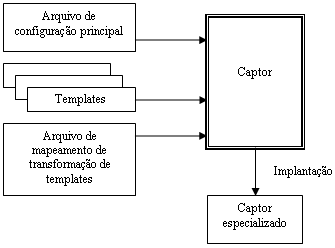
\includegraphics [width=0.55\textwidth] {res/configuring}
  \caption {Arquivos necess�rios para configurar a ferramenta Captor}
  \label{fig:configuring}
\end{figure}

O arquivo de configura��o principal, explicado em detalhes na Sub-se��o \ref{subsec:arqprincipal}, cont�m o meta-modelo da linguagem da especifica��o das aplica��es e as regras de valida��o dessa especifica��o. Os \textit{templates} XSL, explicados em maior detalhes na Sub-se��o \ref{subsec:templatesxsl}, s�o documentos de texto que cont�m marca��es especiais que s�o substitu�das pelos dados da especifica��o da aplica��o durante o processo de gera��o de artefatos. O arquivo de mapeamento de transforma��o de \textit{templates}, explicado em detalhes na Sub-se��o \ref{sec:mapping}, cont�m a informa��o de quais \textit{templates} devem ser transformados no processo de gera��o de artefatos.

%%%%%%%%%%%%%%%%%%%%%%%%%%%%%%%%%%%%%%%%%%%%%%%%%%%%%%%%%%%%%%%%%%%%%%%%%%%%%%%

\subsection{Arquivo de configura��o principal}\label{subsec:arqprincipal}

Na Figura \ref{fig:screenshotCaptor} apresenta-se a interface gr�fica da ferramenta Captor.

\begin{figure} [!ht]
 \centering
  \bfseries
  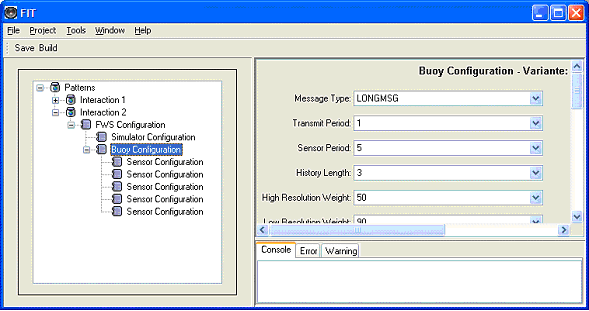
\includegraphics [width=0.9\textwidth] {res/screenshotCaptor}
  \caption {Interface gr�fica da ferramenta Captor}
  \label{fig:screenshotCaptor}
\end{figure}

A ferramenta pode ser configurada para receber especifica��es que s�o armazenadas em formul�rios. Os formul�rios s�o organizados em forma de �rvore e podem ser acessados no painel esquerdo da ferramenta. Cada formul�rio possu� um ou mais componentes gr�ficos que armazenam os dados da especifica��o. Esses componentes gr�ficos podem conter caixas de texto, campos de sele��o, tabelas, entre outros e s�o disponibilizados no painel central-direito da ferramenta.

\textit{\textbf{O arquivo de configura��o principal cont�m o meta-modelo da especifica��o. Esse meta-modelo descreve quais s�o os formul�rios que a ferramenta precisa apresentar, quais componentes gr�ficos cada formul�rio cont�m e quais s�o as regras de valida��o que devem ser verificadas nos dados da especifica��o inseridos nos formul�rios pelo engenheiro de aplica��o.}}

A ferramenta disponibiliza diversos componentes gr�ficos para o engenheiro de dom�nio compor os formul�rios de maneira apropriada. Se o engenheiro de dom�nio precisar de um componente que n�o � parte da biblioteca de componentes de formul�rio padr�o, ele pode utilizar o ``Manual de desenvolvimento de componentes de formul�rio'' para criar novos componentes de formul�rio personalizados. Para realizar a valida��o, a ferramenta disponibiliza dois mecanismos: o mecanismo de valida��o sint�tica e o mecanismo de valida��o estrutural de formul�rios. Os mecanismos de valida��o s�o apresentados nas Subse��es \ref{val1} e \ref{val2} respectivamente.

O primeiro passo na configura��o da ferramenta para um dom�nio espec�fico � a cria��o do arquivo de configura��o principal. Esse arquivo deve ser armazenado no caminho de diret�rio: /install\_dir/domains/nome\_do\_dominio/nome\_do\_dominio.domain, onde /install\_dir representa o caminho de diret�rio da instala��o da ferramenta e /nome\_do\_dominio � o nome do dom�nio da nova configura��o.

Na Listagem \ref{lst:configFileCaptor} � apresentado o conte�do de um arquivo de configura��o simplificado que cont�m o meta-modelo de uma especifica��o que utiliza dois formul�rios. O primeiro formul�rio cont�m uma caixa de texto e uma caixa de sele��o e o segundo formul�rio cont�m uma tabela com quatro colunas.

\lstset{language=xml}
\begin{lstlisting}[caption=Arquivo de configura��o da ferramenta Captor,label=lst:configFileCaptor]
<?xml version=``1.0'' encoding=``UTF-8''?>

<forms>

  <name>SimpleExample</name>

  <form isRoot=``true''>
    <id>1.1</id>
    <enabled>true</enabled>

    <name>Form1</name>
    <variant>Variante1</variant>

    <nextForms>
      <nextForm>
        <id>2.*</id>
        <multiplicity>1</multiplicity>
      </nextForm>
    </nextForms>

    <formComponents>

      <formComponent>
        <fullname>
          captor.windowsystem.formcomponent.textpanel.TextPanel
        </fullname>

        <parameters>

          <parameter>
            <name>id</name>
            <value>textId</value>
          </parameter>
          <parameter>
            <name>label</name>
            <value>Caixa de texto</value>
          </parameter>

        </parameters>

      </formComponent>

      <formComponent>
        <fullname>
    captor.windowsystem.formcomponent.comboboxpanel.ComboBoxPanel
        </fullname>

          <parameters>
  
            <parameter>
              <name>id</name>
              <value>comboId</value>
            </parameter>
            <parameter>
              <name>label</name>
              <value>Caixa de selecao</value>
            </parameter>
          <parameter>
              <name>elements</name>
              <value>1:2:3:4:5</value>
          </parameter>

        </parameters>

      </formComponent>

    </formComponents>

  </form>

  <form>
    <id>2.1</id>

    <enabled>true</enabled>

    <name>Form2</name>
    <variant>Variante1</variant>

    <formComponents>

      <formComponent>
        <fullname>
          captor.windowsystem.formcomponent.tablepanel.TablePanel
        </fullname>

        <parameters>

          <parameter>
            <name>id</name>
            <value>tableId</value>
          </parameter>
          <parameter>
            <name>colname1</name>
            <value>col1</value>
          </parameter>
          <parameter>
            <name>colname2</name>
            <value>col2</value>
          </parameter>

        </parameters>

      </formComponent>

    </formComponents>

  </form>

</forms>
\end{lstlisting}

O documento � formado por uma marca��o ``forms'' que cont�m uma marca��o ``name'' e uma ou mais marca��es ``form''. A marca��o ``name'' cont�m o nome do projeto. Cada marca��o ``form'' representa um formul�rio e pode possuir as marca��es ``id'', ``enabled'', ``name'',  ``variant'', ``help'', ``require'',  ``nextForms'' e ``formComponents'' que devem ser estruturadas nessa ordem respectivamente. As marca��es ``require'' e ``nextForms'' s�o opcionais e as restantes s�o de uso obrigat�rio.

O formul�rio definido na linha 7 possu� o atributo ``isRoot=true''. Apenas um formul�rio pode ter esse atributo com o valor ``true''. Esse atributo indica para a ferramenta que esse ser� o primeiro formul�rio da especifica��o. 

Todos os formul�rios devem possuir um identificador �nico definido na marca��o ``id'' (linhas 8 e 72). O identificar utilizado nos formul�rios deve estar no formato ``NUMERO.NUMERO''. Esse formato � utilizado pela ferramenta no gerenciamento de formul�rios durante o ciclo de vida do projeto.

A marca��o ``variant�� define o nome da variante desse formul�rio. Os formul�rios variantes s�o apresentados na subse��o \ref{subsec:variants}.

A marca��o ``help'' � utilizada para disponibilizar uma breve descri��o de ajuda para o usu�rio engenheiro de aplica��o.

A marca��o ``nextForms'' definida na linha 14 indica que o formul�rio corrente possu� um formul�rio filho identificado pelo id  ``2.*'' (o asterisco indica que o formul�rio filho pode conter os valores: 2.1, 2.2, 2.3 e assim sucessivamente). A marca��o multiplicidade (linha 17) indica qual o n�mero m�ximo de filhos que o formul�rio corrente pode possuir.

A marca��o ``formComponents'' (linha 21) indica quais componentes gr�ficos o formul�rio vai conter. Os componentes de formul�rio s�o definidos em uma ou mais marca��es ``formComponent'' (linhas 23, 43 e 81) e s�o par�metrizados para apresentar comportamento espec�fico. Como exemplo, o componente de formul�rio definido na linha 21 � implementado pela classe: ``captor.windowsystem.formcomponent.textpanel.TextPanel'' e � parametrizado por dois valores (linhas 30 e 34). O par�metro ``id'' representa um identificador �nico para esse componente e o par�metro ``label'' indica qual ser� a etiqueta que ser� disponibilizada ao lado esquerdo do componente gr�fico na interface do formul�rio.

Na Figura \ref{fig:screenshotCaptor2} � apresentado a interface gr�fica da ferramenta Captor configurada com o arquivo apresentado na Listagem \ref{lst:configFileCaptor}.

\begin{figure} [!ht]
 \centering
  \bfseries
  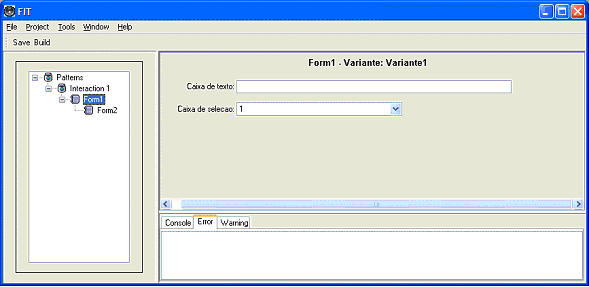
\includegraphics [width=0.9\textwidth] {res/screenshotCaptor2}
  \caption {Interface gr�fica da ferramenta configurada com os dados da Listagem  \ref{lst:configFileCaptor}}
  \label{fig:screenshotCaptor2}
\end{figure}

Os formul�rios ``Form1'' e ``Form2'' podem ser acessados pela �rvore de formul�rios contida no painel esquerdo da ferramenta e os dados dos formul�rios podem ser editados no painel central superior da ferramenta.

Existem diversos componentes gr�ficos de formul�rios disponibilizados junto a ferramenta para compor formul�rios. Cada componente possu� um nome �nico e � desenvolvido para receber diversos par�metros (opcionais e obrigat�rios). A documenta��o desses componentes pode ser encontrada no manual de formul�rios de componentes.

%%%%%%%%%%%%%%%%%%%%%%%%%%%%%%%%%%%%%%%%%%%%%%%%%%%%%%%%%%%%%%%%%%%%%%%%%%%%%%%

\subsubsection{Variantes} \label{subsec:variants}

Um formul�rio pode ter uma variante, ou seja, uma outra vers�o desse formul�rio com pequenas modifica��es. Durante a edi��o da especifica��o, o engenheiro de aplica��o, baseado nos requisitos de software pode selecionar qual variante ele necessita editar.

A Listagem \ref{lst:configFileCaptorExtends} apresenta o trecho do arquivo de configura��o principal que define uma variante para o formul�rio ``Form1'' apresentado na Listagem \ref{lst:configFileCaptor}.

\lstset{language=xml}
\begin{lstlisting}[caption=Defini��o de variantes,label=lst:configFileCaptorExtends]
<form>
  <id>1.2</id>

  <enabled>true</enabled>

  <name>Form1</name>
  <variant>Variante2</variant>

  <extends>1.1</extends>

  <formComponents>

    <formComponent>
      <fullname>
        captor.windowsystem.formcomponent.textpanel.TextPanel
      </fullname>
    </formComponent>

  </formComponents>
		
</form>
\end{lstlisting}

O nome das variantes de um formul�rio deve ter o mesmo nome do formul�rio principal. Como exemplo, os formul�rios identificados por 1.1 e 1.2 possuem o nome ``Form1''. Recomenda-se que o identificador dos formul�rios e seus variantes devem ser iniciados pelo mesmo n�mero, por exemplo, o primeiro variante do formul�rio com identificador 1.1 deve possuir identificador igual a 1.2 e assim sucessivamente.

Na linha 9 da Listagem \ref{lst:configFileCaptorExtends}, a marca��o ``extends'' indica que esse formul�rio vai estender o formul�rio 1.1. As marca��es abaixo da linha 9 sobre-escrevem as marca��es contidas no formul�rio com identificador igual a 1.1. As variantes s�o acess�veis em tempo de execu��o por meio do painel esquerdo da ferramenta.

%%%%%%%%%%%%%%%%%%%%%%%%%%%%%%%%%%%%%%%%%%%%%%%%%%%%%%%%%%%%%%%%%%%%%%%%%%%%%%%

\subsubsection{Valida��o sint�tica}\label{val1}

Os dados inseridos nos componentes dos formul�rios podem necessitar valida��es espec�fcas de dom�nio. Alguns componentes de um formul�rio podem possuir preenchimento obrigat�rio e outros podem ser opcionais. Alguns componentes devem aceitar que o usu�rio insira determinados tipos de dados (inteiro, booleanos, express�es regulares) em seus \textit{widgets} gr�ficos e outros podem aceitar qualquer tipo de valor.

O engenheiro de dom�nio deve parametrizar os componentes de formul�rio para que a ferramenta seja capaz de validar a especifica��o da aplica��o de forma apropriada. Como exemplo, se o engenheiro quiser validar o componente ``captor.windowsystem.formcompo\-nent.textpanel.TextPanel'' da Listagem \ref{lst:configFileCaptor}, ele tem as alternativas apresentadas na Listagem \ref{lst:parameters}.

\lstset{language=xml}
\begin{lstlisting}[caption=Par�metros de valida��o sint�tica do componente TextPanel,label=lst:parameters]
<parameter>
  <name>use</name>
  <value>required</value>
</parameter>

<parameter>
  <name>regexp</name>
  <value>[0-9]+</value>
</parameter>
\end{lstlisting}

O par�matro ``use'' (linha 1) � utilizado para indicar se � necess�rio algum valor na caixa de texto. Se o valor desse par�metro for igual a ``required'', ent�o a ferramenta deve emitir um alerta nos casos em que o usu�rio n�o preencher esse campo.
 
O par�metro ``regexp'' (linha 6) indica que o valor inserido nesse campo de texto deve ter o mesmo valor da express�o regular contida na marca��o ``value''. No exemplo da Listagem \ref{lst:parameters}, a express�o regular ``[0-9]+'' indica que o campo de texto deve possuir um ou mais n�meros inteiros. Qualquer outra combina��o de caracteres � decalrada inv�lida e a ferramenta deve emitir alertas de erros nos casos em que o usu�rio inserir valores incorretos.

Os par�metros de valida��o dispon�veis nos diversos componentes de formul�rios s�o documentados no manual de componentes de formul�rio.

%%%%%%%%%%%%%%%%%%%%%%%%%%%%%%%%%%%%%%%%%%%%%%%%%%%%%%%%%%%%%%%%%%%%%%%%%%%%%%%

\subsubsection{Valida��o estrutural dos formul�rios}\label{val2}

Para obter uma especifica��o completa, o engenheiro pode definir que � necess�rio preencher um n�mero m�nimo de formul�rios. No exemplo da Listagem \ref{lst:configFileCaptor}, se o engenheiro de dom�nio definir que a especifica��o da aplica��o necessita do preenchimento dos formul�rios ``Form1'' e ``Form2'', ele pode inserir a marca��o apresentada na Listagem \ref{lst:require} dentro da especifica��o da formul�rio ``Form1'': 

\lstset{language=xml}
\begin{lstlisting}[caption=Valida��o da estrutura de formul�rios,label=lst:require]
<require>
  <or>
    <formPath>child(2.*)</formPath>
  </or>
</require>
\end{lstlisting}

A marca��o require define quais s�o as depend�ncias entre os formul�rios  e deve ser inserida dentro da marca��o ``form'', entre as marca��es ``variant'' e ``nextForms'' do arquivo de configura��o principal (seria na linha 13 da Listagem \ref{lst:configFileCaptor}).

A marca��o ``require'' pode ter uma ou mais marca��es ``or''. Cada marca��o ``or'' pode ter um ou mais marca��es ``formPath''. A marca��o ``formPath'' deve conter uma express�o que indica o caminho do formul�rio corrente at� o formul�rio que deve estar presente para a valida��o estar completa. Todas as marca��es ``or'' s�o avaliadas em tempo de execu��o e pelo menos uma marca��o ``formPath'' deve ser avaliada como verdadeira para que o formul�rio seja declarado estruturalmente correto. Na tabela \ref{tab:require} s�o apresentados alguns exemplos de express�es que podem definir a hierarquia dos formul�rios.

\begin{table}[ht]
	\centering
	\caption{Valida��o da estrutura de formul�rios}
	\label{tab:require}
		
		\begin{tabular}{|p{200pt}|p{220pt}|}

			\hline 
			\hline 

			\hline 
			child(2.1)&  Este formul�rio deve possuir um formul�rio filho com id igual a 2.1 \\

			\hline 
			parent(1.*) & Este formul�rio deve possuir um formul�rio pai com id igual a 1.*\\

			\hline 
			child(2.*)->child(3.*)->child(4.*) & Este formul�rio deve possuir um formul�rio filho com id igual a 2.* que deve possuir o filho com id igual a 3.* que deve possuir o filho com id igual a 4.* \\

			\hline 
			child(2.*)-> child(3.*)->parent->(2.*) & Este formul�rio deve possuir um formul�rio filho com id igual a 2.* que deve possuir um filho com id igua a 3.* que deve possuir um pai com id igual a 2.* (o �ltimo passo foi propositalmente redundante) \\
			
			\hline 
		\end{tabular}

	\end{table}

%%%%%%%%%%%%%%%%%%%%%%%%%%%%%%%%%%%%%%%%%%%%%%%%%%%%%%%%%%%%%%%%%%%%%%%%%%%%%%%

\subsubsection{Valida��o do arquivo de configura��o principal}

Ap�s o t�rmino da edi��o do arquivo de configura��o principal, o engenheiro de dom�nio pode validar o documento com a ferramenta ``Meta-model validator''. Essa ferramenta l� o arquivo de configura��o principal e caso existam, relata erros e inconsist�ncias. Se o arquivo for validado corretamente pela ferramenta de valida��o de meta-modelos, o gerador pode ser utilizado com a nova configura��o. A ferramenta de valida��o de meta-modelos est� dispon�vel no menu Tools->Meta-Model Validator da janela principal do gerador Captor.

Ap�s a configura��o do meta-modelo (formul�rios e valida��es), a ferramenta ja � capaz de receber a especifica��o da aplica��o, validar essa especifica��o, salvar essa especifica��o em formato XML (esses arquivos s�o chamados de arquivos-fonte) e recuperar essa especifica��o dos arquivos XML e disponibiliza-las nos formul�rios (atividades de criar um projeto, editar o projeto, validar um projeto, fechar o projeto e abrir o projeto de novo).

%%%%%%%%%%%%%%%%%%%%%%%%%%%%%%%%%%%%%%%%%%%%%%%%%%%%%%%%%%%%%%%%%%%%%%%%%%%%%%%

\subsubsection{Gera��o autom�tica do arquivo de configura��o principal}

A ferramenta Captor foi configurada para receber a especifica��o necess�ria para criar o arquivo de configura��o principal e gerar o arquivo de XML com essa especifica��o.

O usu�rio deve abrir a ferramenta, selecionar o menu ``File->Application Project''. Na tela de sele��o de dom�nios o usu�rio deve escolher ``New Captor Project''. Nas telas seguintes o usu�rio deve escolher um diret�rio para os arquivos fontes e um diret�rio para os arquivos de sa�da.

Ap�s o projeto ser criado, o usu�rio pode criar novas intera��es, novos formul�rios e novas variantes. Ap�s a edi��o dos formul�rios o usu�rio pode clicar no bot�o de acesso r�pido ``Build''. Ao t�rmino do processo de transforma��o de artefatos, a ferramenta invoca a ferramenta Ant para realizar a instala��o autom�tica dos novos artefatos.

Ap�s esse processo, o usu�rio pode testar a nova configura��o, selecionando o menu ``File->Application project'' e na primeira tela do \textit{Wizard}, selecionar o dom�nio rec�m criado.

%%%%%%%%%%%%%%%%%%%%%%%%%%%%%%%%%%%%%%%%%%%%%%%%%%%%%%%%%%%%%%%%%%%%%%%%%%%%%%%
%%%%%%%%%%%%%%%%%%%%%%%%%%%%%%%%%%%%%%%%%%%%%%%%%%%%%%%%%%%%%%%%%%%%%%%%%%%%%%%
%%%%%%%%%%%%%%%%%%%%%%%%%%%%%%%%%%%%%%%%%%%%%%%%%%%%%%%%%%%%%%%%%%%%%%%%%%%%%%%

\subsection{Arquivos de \textit{templates} XSL}\label{subsec:templatesxsl}

Um \textit{template} XSL � uma folha de estilos que especifica como um documento de XML deve ser transformado em outro documento. O processo de transforma��o � apresentado na Figura \ref{fig:xslt}.

\begin{figure} [!ht]
 \centering
  \bfseries
  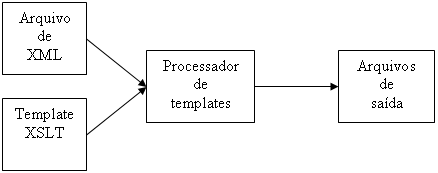
\includegraphics [width=0.7\textwidth] {res/xslt}
  \caption {Transforma��o de \textit{templates} XSL}
  \label{fig:xslt}
\end{figure}

O processador de \textit{templates}, baseado nas instru��es dos \textit{templates}, pode gerar diversos tipos de arquivos de sa�da, dentre eles est�o: arquivos XML, c�digo-fonte, documentos de UML, arquivos de PDF, planilhas e casos de teste.

A ferramenta Captor, armazena as informa��es inseridas na sua interface gr�fica em arquivos no formato XML. Quando o usu�rio solicita a transforma��o da especifica��o em artefatos, a ferramenta recupera os arquivos de XML com o conte�do da especifica��o (arquivos-fonte) e seleciona os \textit{templates} necess�rios para realizar a gera��o de artefatos (o processo de sele��o de \textit{templates} � apresentado na se��o \ref{sec:mapping}).

A estrutura do XML gerado pela ferramenta Captor a partir dos dados da especifica��o possu� uma parte da sua estrutura fixa e uma parte vari�vel. A parte fixa do XML gerado pela ferramenta configurada com a Listagem \ref{lst:configFileCaptor} � apresentado na Listagem \ref{lst:input}.

\lstset{language=xml}
\begin{lstlisting}[caption=Estrutura fixa da especifica��o armazenaa em XML,label=lst:input]
<?xml version=``1.0'' encoding=``UTF-8''?>

 <formsData>

  <project>
    <name>Nome do projeto</name>
  </project>

  <forms>

    <form id=``1.1'' variant=``Default''>

      <data>
      	<!--
      	Os dados armazenados pelos componentes do 
      	formul�rio 1.1 s�o armazenados nesta linha
      	-->
      </data>

      <form id=``2.1'' variant=``Default''>

        <data>
          <!--
          Os dados armazenados pelos componentes do 
          formul�rio 1.2 s�o armazenados nesta linha
          -->
        </data>

      </form>
      
    </form>

  </forms>

</formsData>
\end{lstlisting}

A ferramenta Captor armazena a especifica��o inserida em sua interface gr�fica em uma estrutura de XML que come�a com a marca��o raiz ``data''. Dentro dessa marca��o existem duas marca��es filhas: ``project'' e ``forms''. A marca��o ``project'' (linha 5) cont�m o nome do projeto e a marca��o ``forms'' (linha 9) cont�m os dados da �rvore de formul�rios da especifica��o. A marca��o ``forms'' cont�m uma marca��o ra�z ``form'' (linha 11). Essa marca��o cont�m uma marca��o filho ``data'' (linha 13) e zero ou mais marca��es filhas ``forms'' (nesse caso, uma marca��o na linha 20).

A parte vari�vel da estrutura de diret�rios � armazenada nas marca��es ``data'' filhas da marca��o ``form'' (linhas 11 e 20). Dependendo do n�mero e do tipo de componentes de formul�rio que s�o utilizados para definir um formul�rio, o conte�do dessa marca��o pode variar. Como apresentado na Listagem \ref{lst:configFileCaptor}, o formul�rio ``Form1'' foi configurado para apresentar uma caixa de texto e uma caixa de sele��o (linha 21 e 43 da Listagem \ref{lst:configFileCaptor}). A estrutura de XML que esses dois componentes armazenam as informa��es � apresentado na Listagem \ref{lst:textcombo}.

\lstset{language=xml}
\begin{lstlisting}[caption=Estrutura vari�vel do formul�rio 1.1 definido na Listagem  \ref{lst:configFileCaptor},label=lst:textcombo]
<textatt name=``textId''>
  Valor inserido na caixa de texto
</textatt>
<combo name=``comboId''>
  Valor selecionado da caixa de sele��o
</combo>
\end{lstlisting}

Essa estrutura de XML gerada pelos componentes do Formul�rio ``1.1'' deve ser armazenada na Linha 13 da Listagem \ref{lst:input}. Os formul�rios armazenam os dados de seus componentes em tempo de execu��o. Alguns componentes permitem que a gera��o de XML seja parametrizada. No exemplo da Listagem \ref{lst:textcombo}, o componente TextPanel e o componente ComboPanel utilizam o par�metro ``id'' (linhas 30 e 50 da Listagem \ref{lst:configFileCaptor} respectivamente) para indicar que a ferramenta deve gerar XML personalisado a partir da especifica��o. Esses par�metros foram utilizados pelos componentes de formul�rio para definir o valor do atributo ``name'' (linhas 1 e 4 da Listagem \ref{lst:textcombo}).

Para a obten��o da transforma��o da especifica��o em artefatos de software, o engenheiro de dom�nio que implementa a biblioteca de \textit{templates} deve ter o conhecimento da estrutura do XML gerado pela ferramenta (arquivos-fonte). Ap�s esse conhecimento analisando os arquivos-fonte armazenados em /diretorio\_do\_projeto/input, o engenheiro de dom�nio pode iniciar o processo de desenvolvimento dos \textit{templates}. Os \textit{templates} devem ser armazenados em qualquer caminho de diret�rio abaixo do caminho:  /install\_dir/domains/nome\_do\_dominio /templates e devem ser estruturados de acordo com as regras de trasnforma��o da linguagem XSL.

A linguagen de transforma��es XSL est� fora do escopo desse manual. Instru��es detalhadas da linguagem de transforma��o XSL podem ser encontradas no site: \url{http://www.w3c.org/xslt} e em diversos manuais e livros dispon�veis livremente ou para compra na internet.

%%%%%%%%%%%%%%%%%%%%%%%%%%%%%%%%%%%%%%%%%%%%%%%%%%%%%%%%%%%%%%%%%%%%%%%%%%%%%%%

\subsubsection{Desenvolvimento de \textit{templates} com Zonas de Seguran�a}

Uma zona de seguran�a \cite{herrington} � uma regi�o delimitada por coment�rios onde o desenvolvedor de aplica��es pode inserir c�digo personalisado sem perder as modifica��es com a re-gera��o dos artefatos. 

As marca��es das zonas de seguran�a devem ser escritas nos templates. Ap�s a gera��o dos artefatos, o desenvolvedor pode inserir dados manuais entre as marca��es da zona de seguran�a sem perder os dados com a re-gera��o dos artefatos. Na Listagem \ref{lst:safe2} � apresentado um exemplo de zona de seguran�a que pode ser adicionado a qualquer template processado pela ferramenta Captor.

\lstset{language=java}
\begin{lstlisting}[caption=Exemplo de cria��o de zonas de seguran�a nos arquivos de \textit{template},label=lst:safe2]
// START-SAFE(someSafeZoneId)
  <xsl:value-of select=``/data/safezone[@id= someSafeZoneId]''/>
// END-SAFE
\end{lstlisting}

A cadeia de caracteres ``someSafeZoneId'' deve ser subst�tu�da por um identificador de zonas de seguran�a �nico. Esse identificador � utilizado pela ferramenta para recuperar as informa��es dos arquivos de sa�da.

Na Listagem \ref{lst:safe1} � apresentado um exemplo de zona de seguran�a produzida em um arquivo com c�digo Java gerado pela ferramenta. As modifica��es manuais devem ser inseridas pelo engenheiro de aplica��o abaixo da linha 3 e acima da linha 5.

\lstset{language=java}
\begin{lstlisting}[caption=Exemplo de zonas de seguran�a em arquivos Java,label=lst:safe1]
public void someMethod() {

// START-SAFE(someSafeZoneId)
  System.out.println(``Hello safe-zone!'');
// END-SAFE

  return;
}
\end{lstlisting}

A ferramenta Captor analisa o projeto que est� sendo gerado e caso existam arquivos com zonas de seguran�a que devem ser sobre-escritos no novo processo de gera��o, o conte�do das zonas de segura�a � extra�do dos arquivos que ja foram gerados e � armazenado na �rvore de XML junto com a especifica��o. Durante o processo de transforma��o dos \textit{templates}, esses dados s�o inseridos novamente nos arquivos de sa�da permitindo que o engenheiro de aplica��o personalise o c�digo gerado sem perder essas modifica��es com a re-gera��o dos artefatos.

%%%%%%%%%%%%%%%%%%%%%%%%%%%%%%%%%%%%%%%%%%%%%%%%%%%%%%%%%%%%%%%%%%%%%%%%%%%%%%%
%%%%%%%%%%%%%%%%%%%%%%%%%%%%%%%%%%%%%%%%%%%%%%%%%%%%%%%%%%%%%%%%%%%%%%%%%%%%%%%
%%%%%%%%%%%%%%%%%%%%%%%%%%%%%%%%%%%%%%%%%%%%%%%%%%%%%%%%%%%%%%%%%%%%%%%%%%%%%%%

\subsection{Arquivo de mapeamento da transforma��o dos \textit{templates}}\label{sec:mapping}

O arquivo de mapeamento de transforma��o de \textit{templates} � utilizado pela ferramenta para indicar quais \textit{templates} devem ser utilizados no processo de gera��o de artefatos. Esse arquivo deve ser armazenado no caminho de diret�rio /install\_dir/domains/nome\_do\_dominio/rules.xml, deve ser definido em XML e pode possuir diversas marca��es para controlar o processo de gera��o de artefatos. O conjunto de todas as marca��es poss�veis da ferramenta Captor � chamado de MTL (do ingl�s \textit{Mapping trasnformation language})

Na Listagem \ref{lst:mapping} � apresentado um exemplo simples da estrutura do arquivo de mapeamento para os formul�rios definidos na Listagem \ref{lst:configFileCaptor}.

\lstset{language=xml}
\begin{lstlisting}[caption=Arquivo de mapeamento de \textit{templates},label=lst:mapping]

<composer name=``FIT''>

  <statements>

    <callTask id=``processForm1''/>
    <callTask id=``processForm2''/>
		
  </statements>

  <tasks>

    <task id=``processForm1''>

      <compose>
        <template>grn.st</template>
        <newFilename>\${/data/project/name}_GRN.st</newFilename>
      </compose>

    </task>

    <task id=``processForm2''>

      <compose>
        <template>sql.sql</template>
        <newFilename>sql.sql</newFilename>
      </compose>

    </task>

  </tasks>

</composer>
\end{lstlisting}

O arquivo de mapeamento de \textit{templates} possu� duas marca��es abaixo da marca��o ra�z ``composer'': a marca��o ``statements'' e a marca��o ``tasks''. 

A marca��o ``tasks'' pode ter uma ou mais marca��es ``task''. A marca��o ``task'' � utilizada para definir a transforma��o de um arquivo de template em um arquivo de sa�da. Essa marca��o deve possu�r uma marca��o ``compose''. Cada marca��o ``compose'' � formada pelo nome do arquivo de \textit{template} utilizado na transforma��o (linhas 16 e 25) e pelo nome do arquivo de sa�da que esse \textit{template} transforma (linhas 17 e 26). O caminho de diret�rio dos arquivos de \textit{template}, devem ser indicados de forma relativa ao diret�rio de \textit{templates} do dom�nio (ex: /install\_dir/domains/nome\_do\_dominio/templates). O nome do arquivo que deve ser gerado (marca��o ``newFileName'') pode conter express�es XPATH \cite{xslt} para gerar nomes de arquivos personalisados. Por exemplo, na linha 17 o nome do arquivo gerado ser� o nome contido na marca��o /data/project/name do arquivo fonte concatenado com a cadeia de caracteres ``\_GRN.st''.

A marca��o ``statements'' pode conter tr�s tipos de marca��es: marca��o ``callTask'', ``if'' ou ``for-each''. As marca��o ``callTask'' indica para a ferramenta que uma determinada tarefa deve ser executada (chamadas para a marca��o ``task'' nas linhas 13 e 22).

As marca��es ``if'' s�o utilizadas para realizar assertivas sobre o conte�do do arquivo fonte que est� sendo processado. Na Listagem \ref{lst:conditional} s�o apresentados tr�s exemplos de clausulas condicionais.

\lstset{language=xml}
\begin{lstlisting}[caption=Cl�usulas condicionais no arquivo de mapeamento de \textit{templates},label=lst:conditional]
<statements>

  <if test=``exist(/data/forms/form)''>
    <callTask id=``processForm1''/>
  </if>
  <if test=``equal(/data/forms/form@id='1.1')''>
    <callTask id=``processForm1''/>
  </if>
  <if test=``not-equal(/data/forms/form/='1.1')''>
    <callTask id=``processForm2''/>
  </if>

</statements>
\end{lstlisting}

A primeira clausula da Listagem \ref{lst:conditional} (linha 3) s� � executada se existir o caminho ``/data/forms/form'' no arquivo-fonte (XML gerado a partir da especifica��o da aplica��o), ou seja, a clausula s� � executada  se o formul�rio inicial foi preenchido pelo engenheiro de aplica��o. A segunda clausula condicional (linha 6) s� � executada se o atributo ``id'' da marca��o ``/data/forms/form'' for igual a cadeia de caracteres ``1.1''. A terceira clausula condicional (linha 9) s� � executada se o atributo ``id'' da marca��o ``/data/forms/form'' for diferente da cadeia de caracteres ``1.1''.

O teste realizado pela fun��o ``exists'' recebe como argumento uma express�o XPath. O teste realizado pela fun��o ``equal'' e ``not-equal'' recebe como par�mtros dois argumentos. Os argumentos podem ser uma express�o XPath ou uma cadeia de caracteres delimitada por aspas simples. Se a fun��o da clausula if que est� sendo processada for avaliada como verdadeira, os statemements dentro do if s�o executadas, caso contr�rio as tarefas s�o ignoradas.

As marca��es ``for-each'' s�o utilizadas para realizar intera��es durante o processo de gera��o de artefatos. Na Listagem \ref{lst:next} s�o apresentados exemplos dessas clausulas.

\lstset{language=xml}
\begin{lstlisting}[caption=Cl�usulas ``for-each'' no arquivo de mapeamento de \textit{templates},label=lst:next]
<statements>

  <for-each select=``/data/forms/form/form''>
    <callTask id=``processSomeForm''/>
  </for-each>

  <for-each select=``/data/forms/form/form''>
    <if test=``equal(/data/current/form/@id,'2.1')''>
      <callTask id=``processSomeForm''/>
    </if>
  </for-each>

</statements>
\end{lstlisting}

A marca��o na linha 3 da Listagem \ref{lst:next} indica que a ferramenta deve fazer um loop de transfoma��o em que a chamada callTask da linha 4 � executada o mesmo n�mero de vezes que o n�mero de formul�rios /data/forms/form/form do arquivo-fonte. Al�m da intera��o, essa clausula disponibiliza o n� corrente da �rvore de XML do arquivo-fonte de maneira personalisada por meio do caminho ``/data/current/''. Por exemplo, em cada intera��o da linha 3 da Listagem \ref{lst:next}, a ferramenta realiza uma c�pia do n� /data/forms/form/form no caminho /data/current/form. Essa abordagem � utilizada para que o engenheiro de dom�nio tenha a informa��o, dentro dos templates e dentro do arquivo de mapeamento, sobre qual n� est� sendo processado.

As marca��es dentro da marca��o ``statement'' devem obedecer uma ordem pr�-determinada. Por exemplo, as marca��es ``callTask'' devem ser definidas nas primeiras posi��es. Ap�s as marca��es ``callTask'' todas as marca��es ``ifTask'' devem ser definidas. Ap�s as marca��es ``ifTask'' todas as marca��es ``for-each'' devem ser definidas. Essa ordem � a mesma dentro das marca��es ``ifTask'' ou ``for-each'', ou seja, dentro de uma marca��o ``ifTask'' ou ``for-each'', os ``statements'' devem apresentar a mesma ordem (`�callTask'', ``ifTask'' e ``for-each'').

%%%%%%%%%%%%%%%%%%%%%%%%%%%%%%%%%%%%%%%%%%%%%%%%%%%%%%%%%%%%%%%%%%%%%%%%%%%%%%%

\subsection{In�cio r�pido}

Para o iniciar a configura��o da ferramenta para um dom�nio espec�fico, � necess�rio o planejamento pr�vio sobre qual vai ser a estrutura da especifica��o das aplica��es nesse dom�nio. Ap�s essa fase, execute as seguintes tarefas:

\begin{enumerate}
	\item Fa�a uma c�pia do diret�rio: /install\_dir/domains/Blank para o diret�rio:\\ /install\_dir/domains/foo, onde ``foo'' � o nome do dom�nio escolhido. 
	\item Renomeio o arquivo: /install\_dir/domains/foo/Blank\_.domain para:\\ /install\_dir/domains/foo/foo.domain.
\end{enumerate}

O arquivo /install\_dir/domains/foo/foo.domain representa o arquivo de configura��o principal e possu� a defini��o de um formul�rio com apenas um componente de formul�rio do tipo caixa de texto.

O arquivo /install\_dir/domains/foo/rules.xml � o arquivo de mapeamento de transforma��es e cont�m apenas uma regra que transforma o \textit{template}: /install\_dir/domains/foo\-/template/main.xsl em um arquivo de sa�da.

Os arquivos /install\_dir/foo/pre-build.xml e /install\_dir/foo/pos-build.xml cont�m os esqueletos de um \textit{script} da ferramenta Ant que n�o realiza nenhuma a��o. Esses arquivos podem ser utilizados dessa maneira enquanto n�o for necess�rio nem o pr� e nem o p�s processamento dos arquivos de sa�da.

Para testar a aplica��o, selecione ``File->Application Project''. Na tela inicial do \textit{wizard} selecione o dom�nio ``foo'' e siga as instru��es. Ap�s a cria��o do projeto, clique com o bot�o direito do mouse em cima do item ``Forms'' e selecione no menu o item ``New Interaction''. O primeiro e �nico formul�rio deve aparecer no painel central-direito da ferramenta.

Nesse momento o usu�rio j� pode adicionar texto na caixa de textos do primeiro formul�rio, salvar a aplica��o e gerar um arquivo pressionando o bot�o ``Build''. 

Os arquivos gerados pela ferramenta s�o: /diretorio\_do\_projeto/input/interaction\_0.fit e /diretorio\_de\_saida/interaction\_0/nome\_do\_projeto.nome\_do\_projeto.

O arquivo /diretorio\_do\_projeto/input/interaction\_0.fit cont�m o arquivo de XML gerado pela ferramenta � partir dos dados da especifica��o (arquivo-fonte) e o arquivo /diretorio\_de\_saida/interaction\_0/nome\_do\_projeto.nome\_do\_projeto � o arquivo de sa�da gerado pela ferramenta.

Para continuar o processo de configura��o s�o necess�rios os seguintes passos:

\begin{itemize}

	\item Coloque em um editor de texto os seguintes arquivos:
  \begin{enumerate}
	  \item /install\_dir/domains/foo/foo.domain
	  \item /install\_dir/domains/foo/rules.xml
	  \item /install\_dir/domains/foo/pre-build.xml
	  \item /install\_dir/domains/foo/pos-build.xml
  \end{enumerate}

	\item Alterar os dados do formul�rio ra�z:
	
	\begin{itemize}
		\item Alterar as defini��es do primeiro formul�rio.
		\item Adicionar mais componentes no formul�rio ra�z.
		\item Adicionar mais formul�rios.
		\item Adicionar as restri��es de valida��o necess�rias.
	\end{itemize}
	
	\item Examinar a estrutura dos arquivos-fonte gerados pela ferramenta e realizar o desenvolvimento dos \textit{templates}.
	\item Alterar o arquivo de mapeamento de \textit{templates}.
	\item Testar a nova configura��o.
\end{itemize}

Se o usu�rio desejar gerar automaticamente o arquivo de configura��o principal, ele deve criar um novo projeto por meio do menu ``File->Application Project'' e na tela inicial do \textit{wizard} selecionar ``New Captor Project''. No nome do projeto, o usu�rio deve digitar ``foo'' (``foo'' � o nome do dom�nio escolhido).

Ap�s a cria��o do projeto o usu�rio pode criar e editar novos formul�rios e ao fim do processo clicar no bot�o ``Build''. O processo de gera��o sobre-escreve o arquivo de configura��o principal /install\_dir/domains/foo/foo.domain pelo arquivo que foi gerado. Os arquivos de mapeamento e de pre e pos processamento n�o s�o alterados no processo autom�tico.

%%%%%%%%%%%%%%%%%%%%%%%%%%%%%%%%%%%%%%%%%%%%%%%%%%%%%%%%%%%%%%%%%%%%%%%%%%%%%%%


\section{Utiliza��o da ferramenta}\label{sec:utilizacao}
\noindent A ferramenta Captor fornece apoio para a cria��o e edi��o de projetos. Cada projeto � definido por um nome, um diret�rio onde a especifica��o � armazenada e um diret�rio onde os arquivos de sa�da s�o armazenados ap�s a gera��o dos artefatos.

Na Figura \ref{fig:interaction} � apresentado a utiliza��o da ferramenta Captor, configurada com o arquivo de configura��o principal apresentado na Listagem \ref{lst:configFileCaptor}.

\begin{figure} [!ht]
 \centering
  \bfseries
  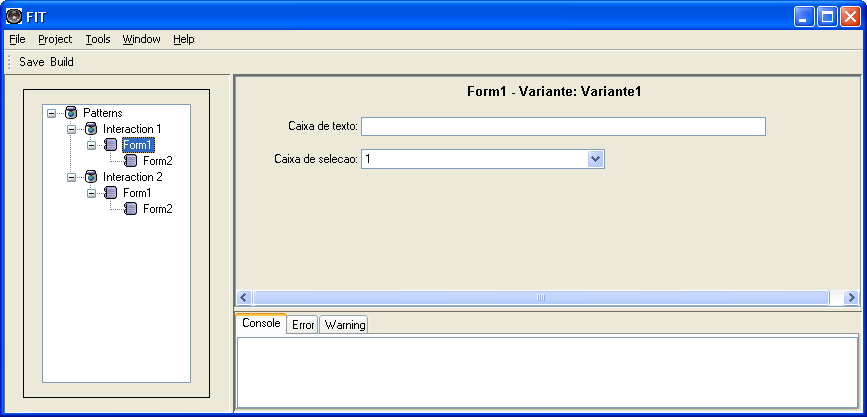
\includegraphics [width=0.9\textwidth] {res/interaction}
  \caption {Utilizac�o da ferramenta Captor}
  \label{fig:interaction}
\end{figure}

Em um projeto, o engenheiro de aplica��o pode editar uma ou mais especifica��es por meio de uma ou mais �rvores de formul�rios. O usu�rio pode editar diversas �rvores de formul�rios por meio de diversas intera��es. Cada intera��o possu� uma �rvore de formul�rios que define a especifica��o de uma aplica��o. 

Na Figura \ref{fig:interaction} � apresentado a interface da ferraenta Captor sendo utilizado para editar duas especifica��es. O  engenheiro de aplica��o criou duas intera��es que podem ser acessadas pelos elementos ``Interaction 1'' e ``Interaction 2'' do menu da barra esquerda da ferramenta. Durante a transforma��o dos artefatos, os arquivos de sa�da dessas especifica��es s�o armazenados no caminho de diret�rio: /output\_dir/interaction\_0 e /output\_dir/interaction\_1, onde /output\_dir � o diret�rio de sa�da que � definido no momento em que o engenheiro de aplica��o cria um projeto na ferramenta Captor.

\subsection{Pre e Pos transforma��o de artefatos}

O Ant \cite{ant} � uma ferramenta que auxilia na compila��o e instala��o de projetos Java. Essa ferramenta oferece diversas funcionalidades para a instala��o de aplica��es Java e n�o Java, tais como: copiar arquivos, apagar arquivos, mover arquivos, compactar arquivos em diversos formatos, integra��o com mecanismos de controle de vers�o, execu��o de aplicativos externos,  compila��o autom�tica de aplicativos Java, entre outras funcinalidades.

A ferramenta Captor pode ser configurada para realizar o processamento dos arquivos com a ferramenta Ant antes e depois do processo de transforma��o de artefatos. Se existir um arquivo do Ant com o nome /install\_dir/domains/nome\_do\_dominio/pre-build.xml o Ant ser� chamado com esse arquivo como par�metro antes da ferramenta executar a transforma��o dos artefatos. Se existir um arquivo do Ant com o nome ``/install\_dir/domains/ nome\_do\_dominio/pos-build.xml'' o Ant ser� chamado com esse arquivo como par�metro depois da ferramenta executar a transforma��o dos artefatos. 

Se o engenheiro de aplica��o achar necess�rio, ele pode criar os arquivos de pre e pos transforma��o no diretorio: /diretorio\_do\_projeto/pre-build.xml  e ``/diretorio\_do\_projeto/ pro-build.xml'', onde o diret�rio /diretorio\_do\_projeto representa o caminho de diret�rio selecionado para armazenar os arquivos do projeto durante a cria��o de projeto. Se esses arquivos existirem, a ferramenta cancela as execu��es do Ant que utilizam os \textit{scripts} contidos no diret�rio de dom�nio e executa o Ant com esses arquivos do diret�rio de projeto.

O \textit{script} do Ant n�o pode obter informa��es sobre os dados do projeto que est� sendo transformado previamente. Para poder copiar ou mover arquivos de posi��o, o Ant deve ter o conhecimento do local de sa�da dos diret�rios transformados pela ferramenta Captor, entre outras informa��es. Para resolver esse problema, o usu�rio pode inserir as linhas contidas na Listagem \ref{lst:antNone} no \textit{script} do Ant.

\lstset{language=xml}
\begin{lstlisting}[caption=Pr�-processamento do \textit{script} do Ant,label=lst:antNone]
<!--PROJECT\_GENERATED\_DATA - DO\_NOT\_EDIT-->
<!--PROJECT\_GENERATED\_DATA - DO\_NOT\_EDIT-->
\end{lstlisting}

Antes de executar o Ant, a ferramenta Captor realiza o pre-processmento dos arquivo   de pre e pos transforma��o para criar as seguintes vari�veis:

\lstset{language=xml}
\begin{lstlisting}[caption=Resultado do pr�-processamento do \textit{script} do Ant,label=lst:antFull]
<!--PROJECT_GENERATED_DATA - DO_NOT_EDIT-->
<property name=``install_path'' location=``/Captor''/>
<property name=``project_name'' value=``FWS1''/>
<property name=``project_path'' location=``/Captor/projects/foo''/>
<property name=``project_output_path'' location=``/output''/>
<property name=``interaction_0'' value=``0''/>
<property name=``interaction_1'' value=``1''/>
<!--PROJECT_GENERATED_DATA - DO_NOT_EDIT-->
\end{lstlisting}

A variavel ``install\_path'' indica o local de instala��o da ferramenta Captor. A vari�vel ``project\_name'' indica o nome do projeto, as vari�veis ``project\_path'' e ``project\_output\_path'' indicam o diret�rio do projeto e o diret�rio para onde os arquivos trasnformados s�o armazenados. As vari�veis ``interaction\_X'' indicam quantas intera��es foram editadas na ferramenta.

Uma das principais funcionalidades da ferramenta Ant utilizada em conjunto com a ferramenta Captor � a copia autom�tica dos arquivos de sa�da para o diret�rio de arquivos de desenvolvimento ou, se o usu�rio utilizar zonas de seguran�a o Ant pode ser executado para copiar os arquivos modificados manualmente do diret�rio de desenvolvimento para o diret�rio de sa�da do gerador antes que o processo de transforma��o seja iniciado.



%%%%%%%%%%%%%%%%%%%%%%%%%%%%%%%%%%%%%%%%%%%%%%%%%%%%%%%%%%%%%%%%%%%%%%%%%%%%%%%

\subsection{Mensagens de erro durante a valida��o da especifica��o e os seus significados}

Diversas mensagens de erro de valida��o podem aparecer no painel de visualiza��o de erros enquanto o engenheiro de dom�no edita a especifica��o da aplica��o. \footnote{Se o painel de visuaaliza��o de erros n�o estiver aparecendo, clique no menu Windows->Show View->Error.}.

Existem dois tipos de erros de valida��o: os erros de falha na valida��o de um formul�rio e os erros de checagem estrutural. Nas Subsec��es \ref{subsec:m1} e \ref{subsec:m2} s�o apresentados detalhes de como interpretar essas mensagens de erro.

%%%%%%%%%%%%%%%%%%%%%%%%%%%%%%%%%%%%%%%%%%%%%%%%%%%%%%%%%%%%%%%%%%%%%%

\subsubsection{Erros de valida��o de formul�rios}\label{subsec:m1}

Os dados inseridos nos formul�rios precisam ser validados. Quando o usu�rio insere um dado incorreto em algum campo do formul�rio, a ferramenta emite uma mensagem de erro avisando o usu�rio que n�o foi poss�vel validar a especifica��o corretamente.\\

\textbf{Mensagem:} Form validation error\\

\textbf{Sa�da de exemplo:}\\

\textit{Error in form: Interaction 1->Form1}\\

\textit{Message error:} \\

  \textit{* Age is not a number.}\\

\textbf{Significado:}\\

	A linha ``Error in form: Interaction 1->Form1'' indica em qual formul�rio ocorreu o erro. Nesse caso, o erro ocorreu no formul�rio ra�z com nome igual a ``Form1'' localizado na intera��o 1.
	
	A mensagem de erro ``Age is not a number'' indica que o campo de idade n�o possu� um valor v�lido.

%%%%%%%%%%%%%%%%%%%%%%%%%%%%%%%%%%%%%%%%%%%%%%%%%%%%%%%%%%%%%%%%%%%%%%

\subsubsection{Erros de checagem estrutural}\label{subsec:m2}

Para obter uma especifica��o completa, alguns formul�rios podem ter o preenchimento obrigat�rio. Se o usu�rio n�o preencher todos os formul�rios obrigat�rios, a ferramenta deve emitir uma mesangem de erro notificando o usu�rio. \\

\textbf{Mensagem:} Structural form validation error\\

\textbf{Output de exemplo:}\\

\textit{The form: Interaction 1->Form1 require one of these forms:} \\

\textit{child(Form2) or child(Form3)->child(Form4)}\\

\textit{AND}\\

\textit{child(Form5)}\\

\textit{Insert the required forms indicated above to get a valid specification.}\\

\textbf{Significado:}\\

A linha ``The form: Interaction 1->Form1 require one of these forms:'' indica que o formul�rio ra�z com nome igual a ``Form1'' da intera��o 1, possu� uma depend�ncia obrigat�ria com os formul�rios indicados na mensagem de erro.

Os formul�rios que devem ter preenchimento obrigat�rio s�o especificados nas regras l�gicas da mensagem. Nesse caso, o formul�rio ra�z Form1 da intera��o 1 deve possuir:\\

	(\textit{um filho com nome igual a Form2} \textbf{OU} \textit{um filho com nome igual a Form3 que deve possuir um filho com nome igual a Form4}) \textbf{E} (\textit{um filho com nome igual a Form5}).
	
%%%%%%%%%%%%%%%%%%%%%%%%%%%%%%%%%%%%%%%%%%%%%%%%%%%%%%%%%%%%%%%%%%%%%%



%******************  Bibliografia  ********************************************

\newpage
\renewcommand{\bibname}{Refer�ncias}
\bibliography{res/refs}

\addcontentsline{toc}{section}{\bibname}

%***************************************

\end{document}
